\section{Detector Calibration}
To identify valid neutron events and precisely determine the TOF start (micropulse start 
time) and TOF stop time (arrival at TOF detector) for each event, a series of corrections 
are required.  First, each event was assigned to the correct macropulse.
Time offsets (accounting for cable and
electronics delay) were applied, coarsely synchronizing all detectors with
facility-provided pulses indicating the arrival time of proton micropulses on the
tungsten target, so-called ``T$_{0}$" pulses.
To improve the detector- and digitizer-associated timing resolution for each TOF
event, the digitized waveform for each event was passed 
through an offline software CFD algorithm, improving the timing resolution 
for TOF-detector events to 0.52 ns FWHM (see Figs. \ref{LRTimeDifferenceLinear}
and \ref{DifferenceThresholdsFit}).

\begin{figure*}
    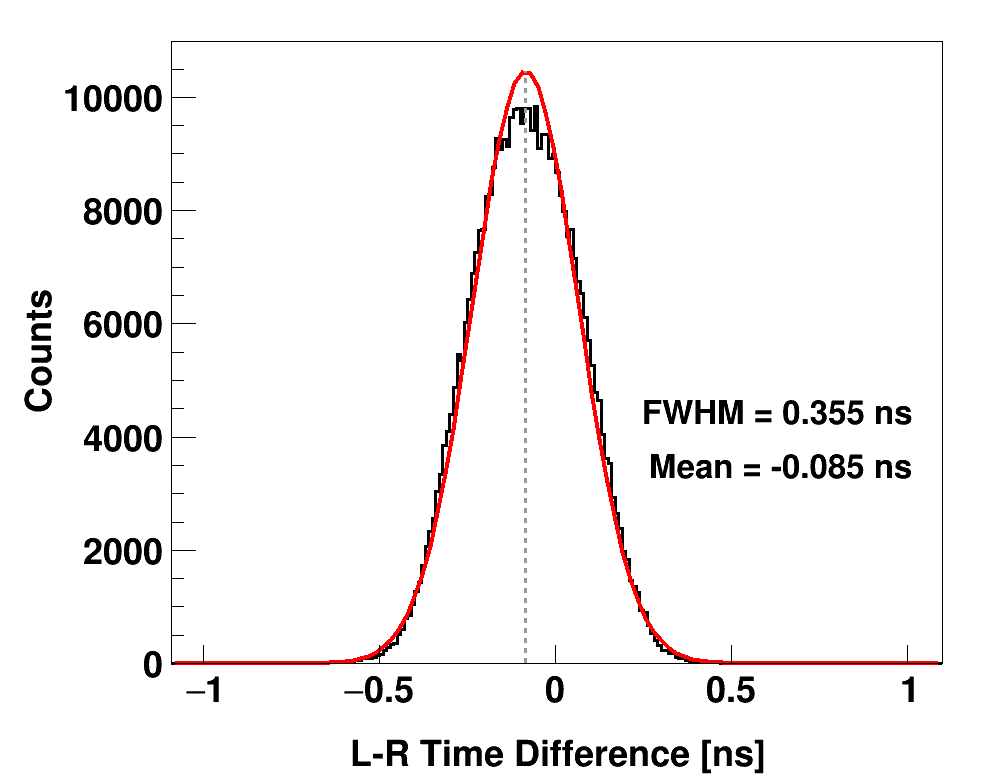
\includegraphics[scale=0.3]{figures/Difference_Linear.png}
    \caption{Time difference between left and right PMTs of time-of-flight detector}
    \label{LRTimeDifferenceLinear}
\end{figure*}

(Color online) For all events in a diagnostic data run, the time difference   
        between the left and right PMTs of the TOF detector is plotted.
        A Gaussian fit (in red) to these events reveals an 85-ps delay of the right PMT with 
    respect to the left PMT and a left-right time difference FWHM of 355 ps.

\begin{figure*}
    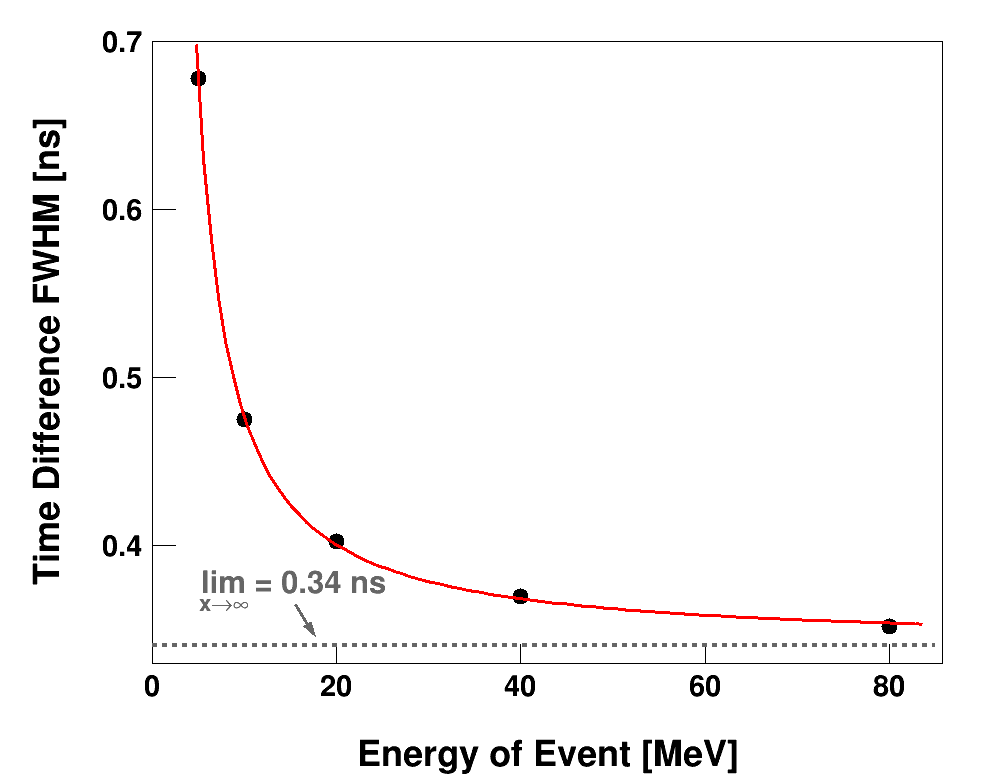
\includegraphics[scale=0.3]{figures/DifferenceThresholdsFit.png}
    \caption{Intrinsic time resolution of time-of-flight detector as a function of signal amplitude}
    \label{DifferenceThresholdsFit}
\end{figure*}

(Color online) The time difference between the left and right PMTs
        of the TOF detector was calculated for all events in a diagnostic run.
        The FWHM of these time differences as a function of
        neutron energy are shown (black points) and fitted with a hyperbolic
        curve (red line). For low-energy
        events, the time resolution is poorer due to the lower signal amplitude and
        the larger traversal time for neutrons through the 1-inch detector. As energy
        increases, the FWHM time resolution approaches an asymptote of 0.34
    ns (grey dashed line).

To improve the micropulse time resolution and test the stability of the
micropulse period during a macropulse, all $\gamma$ rays for a given macropulse
were identified and their average TOF calculated. The difference between this
time and the expected TOF (given the TOF detector distance and speed of light)
was applied to all events in that macropulse (see Fig.
\ref{TimingCorrectionStudy}). After these corrections, the total TOF resolution
(the FWHM of the $\gamma$-ray peak in the TOF spectra) ranged from
0.60-0.85 ns over the series of \tot\ measurements and is comparable to the resolution from 
our digitizer-mediated Ca experiment from 2008 \cite{Shane2010}.
To contextualize, for a 100-MeV neutron and a TOF detector distance of 27 meters, a TOF 
uncertainty of 0.80 ns translates to an energy resolution of $\approx$900 keV.
For neutrons below $\approx$20 MeV, the TOF time resolution worsens as the traversal time 
through the 1-inch thickness of the TOF detector becomes non-negligible.
However, because the TOF of these neutrons is already several hundred ns or
longer, the relative energy resolution ($\frac{\Delta E}{E}$) is
superior at low energies: for a 5 MeV neutron with a 0.82 ns detector-traversal time and
an inherent TOF resolution of 0.80 ns, $\Delta E$ is 13 keV. These energy uncertainties
have been propagated through subsequent analysis into our \tot\ results below.

\begin{figure}
    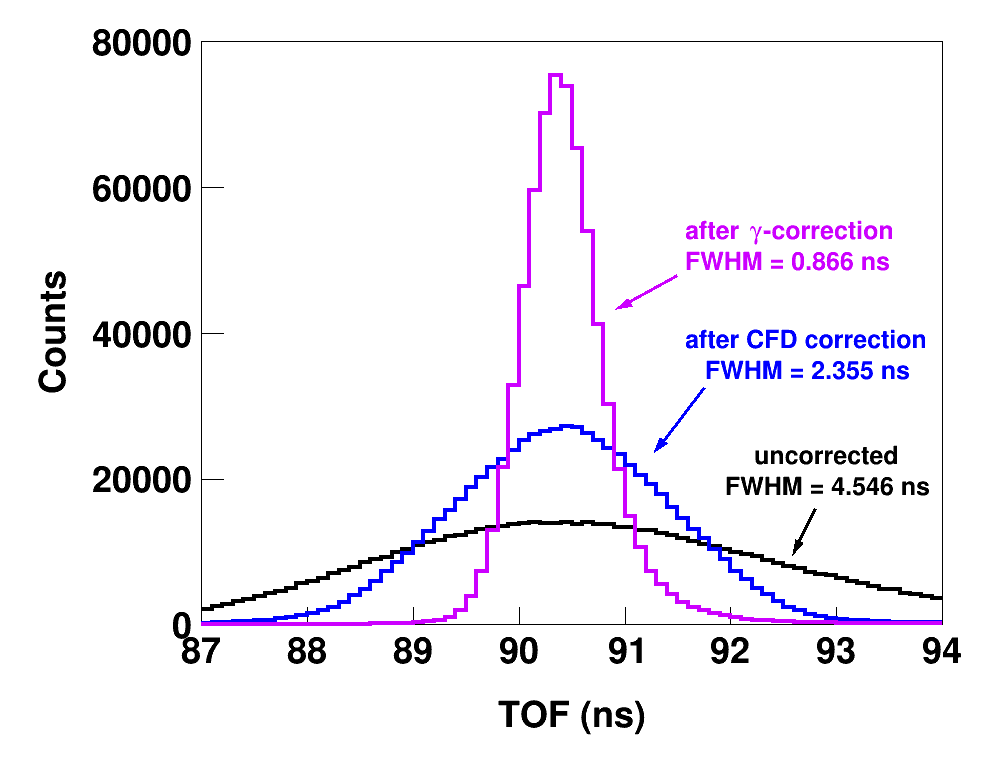
\includegraphics[scale=0.24]{figures/TimeCorrections.png}
    \caption{Improving timing precision with a software CFD and $\gamma$-ray averaging}
    \label{TimingCorrectionStudy}
\end{figure}

(Color online) The effects of timing corrections on the $\gamma$-ray
        peak of a typical run are shown. The uncorrected spectrum is shown in black,
        the spectrum after correction with our software CFD is shown in blue,
        and the spectrum after correction with both our software CFD and
        $\gamma$-averaging is 
        shown in pink. For this run, the final $\gamma$-ray peak 
        FWHM after both corrections is 0.866 ns, comparable to the precision we
        achieved in our Ca study \cite{Shane2010}, which also employed $\gamma$-
        averaging.

Precise determination of the TOF distance was done by comparing our measured \tot\ data
for $^{\text{nat}}$C with that from literature from 3-15 MeV, the results of which are
shown in Fig. \ref{DistanceStudy}. The distance was determined as [insert
updated value]$\pm$1 cm for the Ni and Rh measurement and [insert updated value]$\pm$1 cm 
for the Sn and O measurement.


\section{Energy Determination from Time-Of-Flight}
\begin{figure*}
    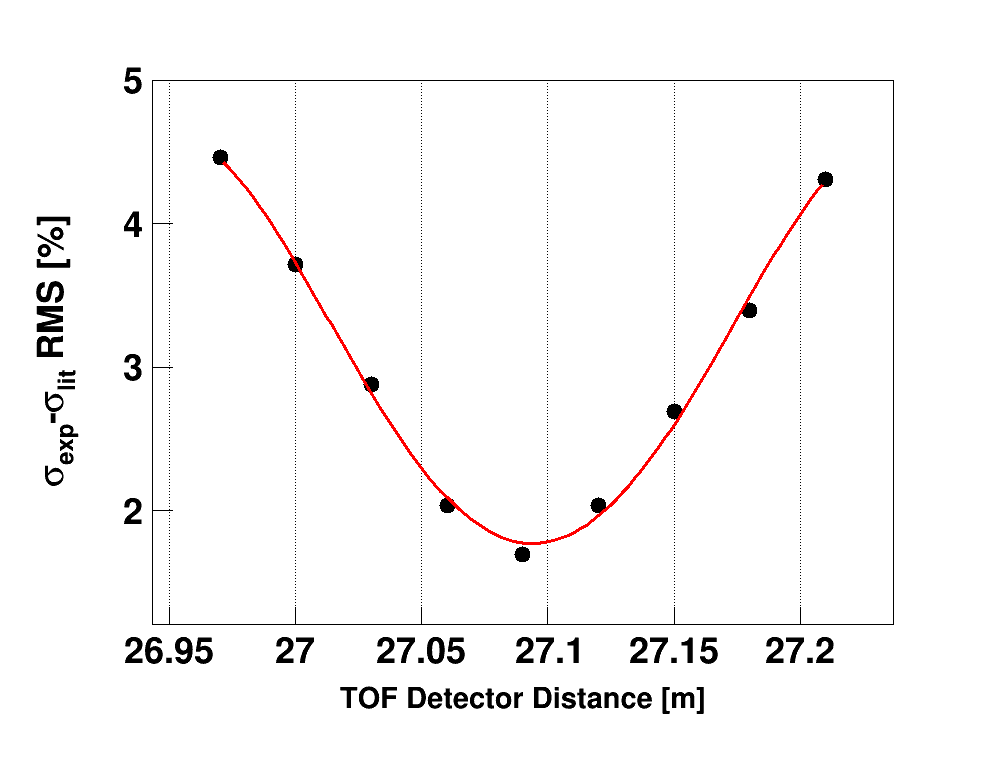
\includegraphics[scale=0.3]{figures/DistanceStudyNi.png}
    \caption{Determining the time-of-flight detector distance using \cNat\ resonances}
    \label{DistanceStudy}
\end{figure*}

(Color online) Results of a study to determine the distance between
    the neutron source and the TOF detector for the Ni/Rh running configuration
are shown. First, a plausible range of flight path distances (26.97-27.21 m) was
selected based on rough estimation during the experiment. Using each
distance in this range, the \tot\ for natural carbon was calculated in the
resonance region (3-15 MeV). The RMS difference between the cross section
generated using that distance and literature data from Abfalterer
\cite{Abfalterer2000, Abfalterer2001} was calculated (shown as black points in
the figure). A quartic fit to these RMS data is shown (solid line). By minimizing the
RMS difference, the flight path distance of 2709$\pm$1 cm was determined.

\begin{figure*}
    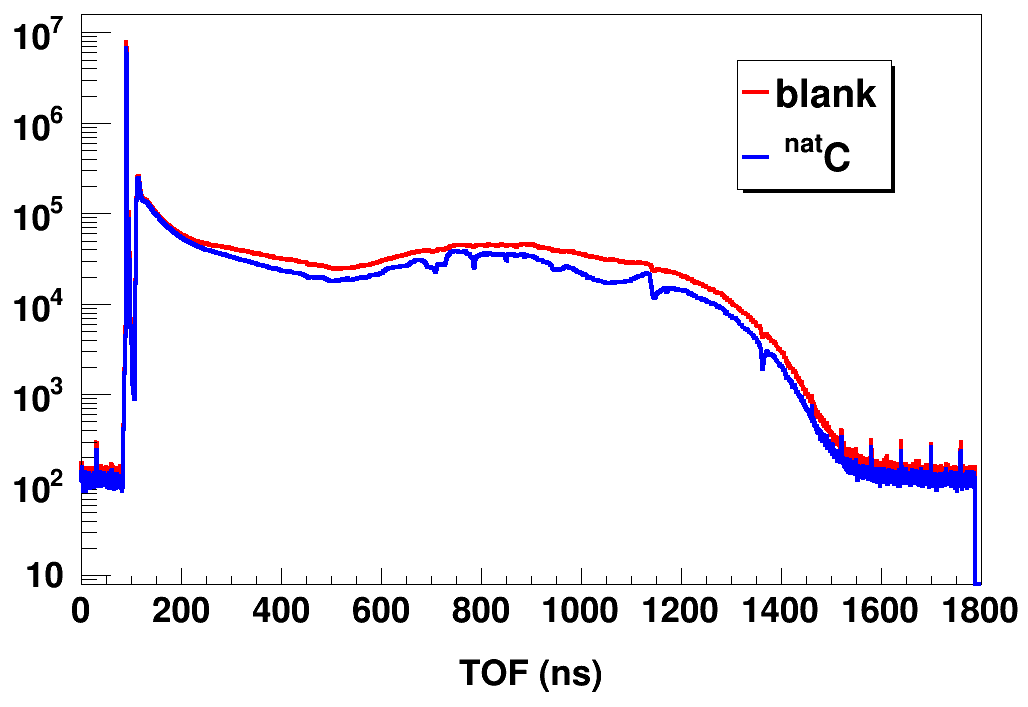
\includegraphics[scale=0.3]{figures/exampleTOFSpectrum.png}
    \caption{Typical time-of-flight spectra for the \cNat\ sample and the blank}
    \label{ExampleTOFSpectrum}
\end{figure*}

(Color online) TOF spectra after analytic deadtime correction and
        veto and integrated charge gating for the blank sample (in
        red) and for the $^{\text{nat}}$C sample (in blue), from the Ni/Rh experiment.
        The $\gamma$-ray peak is visible as a sharp spike at 90 ns, followed by
        the highest-energy neutrons at 130 ns. The small spikes spaced 60 ns
        apart (visible before 90 ns and after 1500
        ns) are identified as $\gamma$-ray peaks from a low-level, continuous ``drip" 
        of protons onto the tungsten target caused by mistuning of the proton 
        buncher; their effect on the calculated cross sections is negligible.

\section{Deadtime Correction}
Because events are not processed instantaneously, there is a brief period
after each trigger during which the digitizer is busy processing that trigger.
Any newly-arriving events in this period will be ignored,
privileging events arriving earlier and thus distorting
TOF spectra and resulting cross sections. This busy period is referred to as the
``analytic" or ``per-event" deadtime and can be corrected for according to standard 
techniques
\cite{Moore1980}. Assuming negligible variation in beam flux between micropulses
(an assumption investigated below), the fraction of time $F[i]$ that the digitizer is dead 
for a given time bin $i$ can be calculated:
\begin{equation}
    F_{i} = \sum^{N-1}_{j=0} R_{(i-j)\text{ mod N}}\times P_{j}
\end{equation}
where $N$ is the number of time bins in the micropulse, $R_{x}$ is the rate of
detected events per micropulse in bin $x$, and $P_{j}$ is the probability that the
digitizer is still busy from a trigger $j$ bins ago. To model $P_{j}$, we
employed a logistic function and fitted it to the observed spectrum for time
differences between consecutive events (see Fig.
\ref{TimeDifferenceBetweenEvents}). For a given bin $i$, the fraction of time that the 
digitizer is dead, $F_{i}$, is in essence a discrete convolution of the
\textit{measured} TOF spectrum with $P_{j}$. Note that except for the first and
last micropulses in a macropulse, micropulses are consecutive and thus deadtime effects can
``wrap around" from the end of one micropulse to the next. For these wrap-around
contributions (that is, $j>i$), the (mod N) term ensures that the bin referred
to by $i-j$ is non-negative and has physical meaning as a time bin from the previous 
micropulse.

Because trigger processing is done quickly in
firmware onboard the digitizer, the per-event deadtimes affecting our
measurement ranged from 150-230 ns. For a 230 ns deadtime, the probability-dead
$F_{i}$ of our time bins is given in Fig.
\ref{ExampleDeadtimeSpectrum}, showing that the probability-dead never exceeds
25\%, much smaller than the 50-80\% of previous analog experiments \cite{Finlay1993,
Abfalterer2001}.
Once the fraction dead was identified for each time bin, the total number of
events detected in that bin, $N_{m}[i]$, was corrected to the \textit{true}
number of events in that bin $N_{t}[i]$ that would have been detected in the
absence of a
per-event deadtime:
\begin{equation}
    N_{t}[i] = -ln\left(\frac{1-\frac{N_m[i]}{M}}{(1-F_{i})\times M}\right)
\end{equation}
where M is the total number of micropulse periods. The difference between
uncorrected and analytic-deadtime-corrected TOF spectra is shown in Fig.
\ref{CorrectionEffectOnTOF}. At large TOFs (low energies) the correction is as low as a
few percent, but at small TOFs (high energies) when the digitizer is still dead
from the $\gamma$-ray flash and high-energy neutrons, the correction is significant
($\approx$20\% for our Ni/Rh runs, and $\approx$40\% for our Sn/O runs). These 
corrections are themselves far lower than the typical
analytic deadtime correction required when using analog approaches \cite{Finlay1993,
Abfalterer2001} that were as high as 500\%.% The effect of this correction on the final 
%cross section results is shown in Fig. \ref{DeadtimeEffectOnCS}.

[insert information about constant rate and discarding first 40 micropulses]

\begin{figure}
    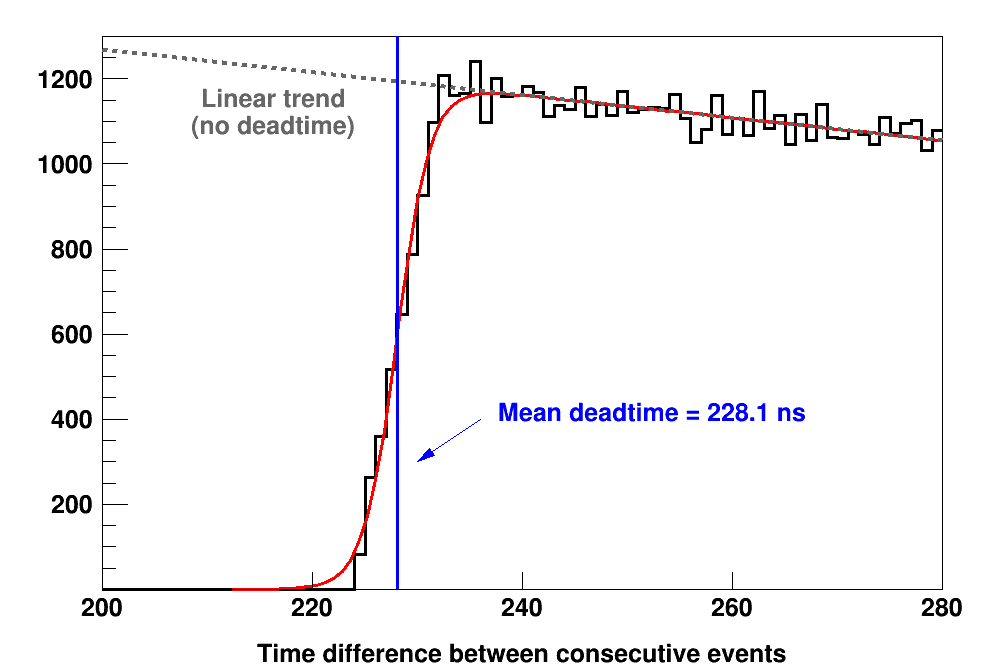
\includegraphics[scale=0.24]{figures/TimeDifferenceBetweenEvents.png}
    \caption{The time difference between consecutive events in the time-of-flight detector}
    \label{TimeDifferenceBetweenEvents}
\end{figure}

The time difference between adjacent TOF-detector
    events for a single run is plotted (black histogram). Below a certain
minimum time difference (the ``deadtime"), no events are recorded. A logistic
fit (red) models the detector's deadtime response and is used to generate a
deadtime correction. The underlying linearly-decreasing count rate (gray dashed
line) in incorporated into the logistic model. From the fit, a mean deadtime of
228.1 ns was extracted for the Sn and O run configurations (a similar
procedure was used to recover a deadtime of [insert deadtime] for the Ni and Rh
run configurations).

\begin{figure*}
    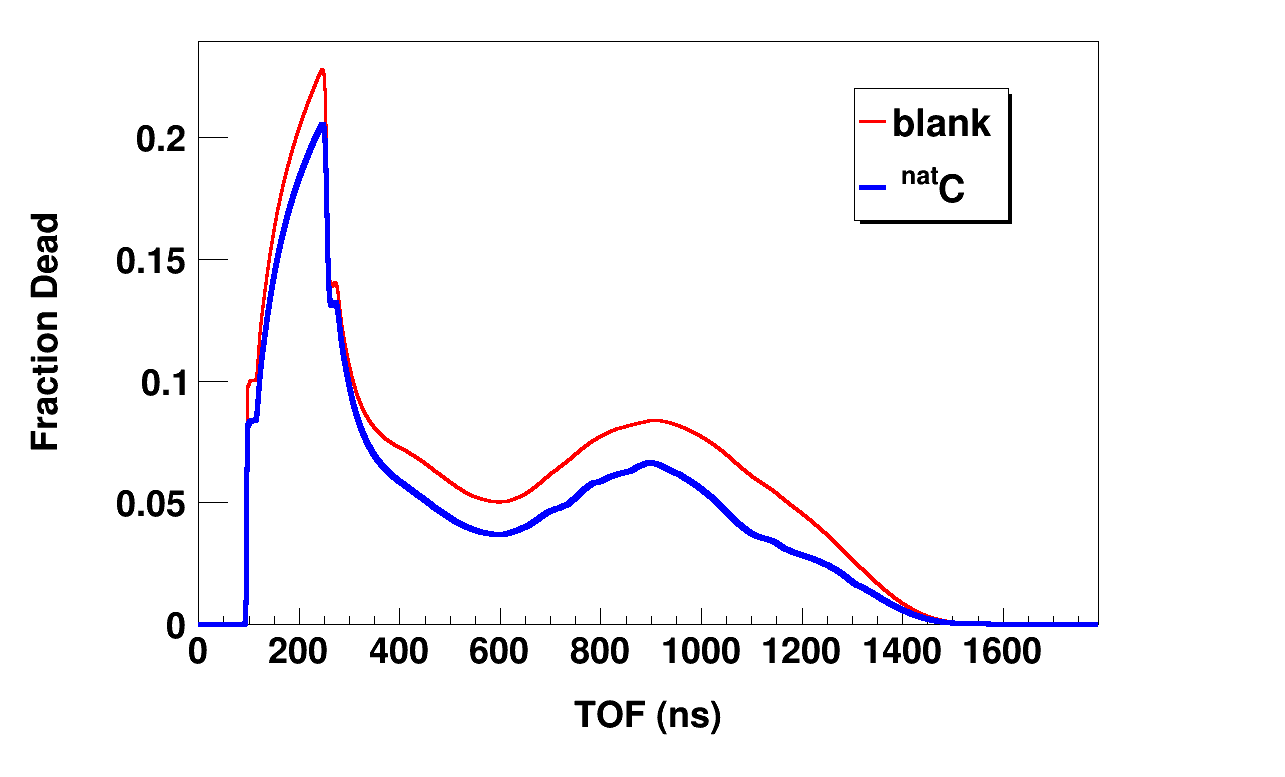
\includegraphics[scale=0.3]{figures/exampleDeadtimeSpectrum.png}
    \caption{Digitizer busy probability as a function of time within micropulse}
    \label{ExampleDeadtimeSpectrum}
\end{figure*}

(Color online) Using TOF data from a typical run, the probability that a given 
        TOF bin is ``dead" is shown for the blank sample (dashed line) and the $^{\text{nat}}$C   
        sample (solid line). The sharp rise at 90 ns is the response to the
        $\gamma$-ray flash, the gradual increase from 90-245 ns is the response to
        the arrival of high-energy neutrons, and the sharp fall at 245 ns
        is the elapse of the $\gamma$-ray ``shadow". Only high-energy neutrons
        have a probability-dead exceeding 10\%.

\begin{figure*}
    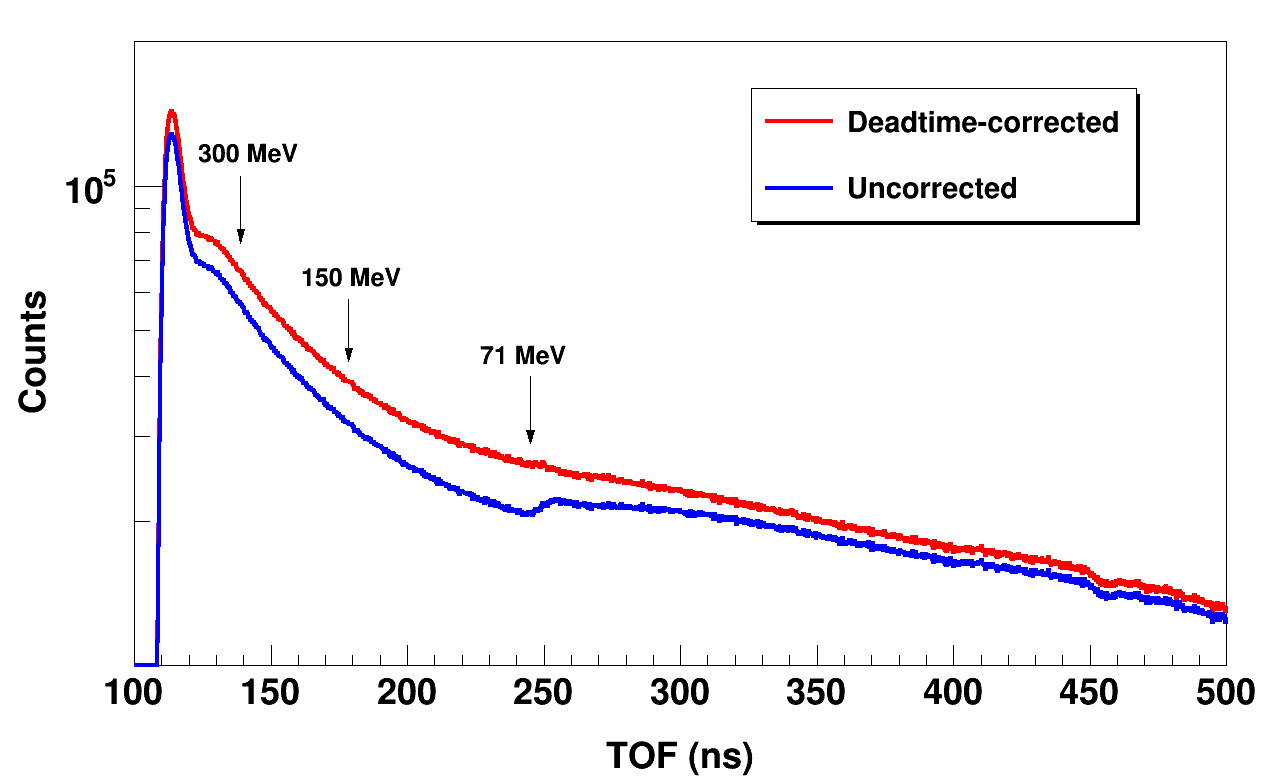
\includegraphics[scale=0.3]{figures/CorrectionEffectOnTOF.png}
    \caption{The effect of deadtime correction on a typical time-of-flight spectrum}
    \label{CorrectionEffectOnTOF}
\end{figure*}

(Color online) A typical TOF spectrum from the Ni/Rh
        run configuration is shown, before (in blue) and after (in red) analytic
        deadtime correction. Relevant neutron energies are indicated above the spectra.
        For this digitizer configuration, the mean deadtime was 155 ns (see Fig.
        \ref{TimeDifferenceBetweenEvents} for details on mean deadtime determination).
        Note that at 245 ns, there is an
        obvious defect in the uncorrected spectrum is repaired in the corrected
        spectrum. The defect
        corresponds to the elapse of the 155-ns-long deadtime ``shadow" from the $\gamma$-ray
        flash, which arrived at 90 ns (not shown).

In addition to analytic deadtime, an additional deadtime associated with digitizer readout 
to the data acquisition computer (DAQ), was identified. Each pair of
digitizer channels shares a common buffer for storing events; upon reaching a
user-defined threshold, buffer contents are read out to the DAQ as packets.
During readout, the digitizer is ...something.
This is likely the largest source of systematic error in our measurement.

During analysis, it was noted that occasionally (1 in 400 macropulses), one or two 
adjacent macropulses would have an abnormally small number of flux monitor events or 
TOF events. The frequency of these ``data dropouts" was similar to the rate of
switching between DPP and waveform modes and we suspect it is related to edge
case behavior right before or after a mode switch. To mitigate this issue,
any macropulse that had less than 50\% of the average event rate in either the
flux monitor or TOF detector channel was ignored during cross section calculation.

After applying these corrections, the veto and integrated charge gates are applied to 
all events and surviving events are populated into TOF spectra (see Fig.
\ref{ExampleTOFSpectrum}). Next, room background was subtracted (responsible for 0.1\% to 
1\% of event rate, depending on energy) and spectra were mapped to the energy domain.

\section{Cross Section Calculation}
The fundamental quantity of interest, \tot, is related to the flux
loss through a sample by:
\begin{equation}
I_{t} = I_{0}e^{-{\ell\rho\sigma_{tot}}}
\end{equation}
or, equivalently,
\begin{equation}
    \tot = -\frac{1}{\ell\rho}ln\left(\frac{I_{t}}{I_{0}}\right)
\end{equation}
where $I_{0}$ is the neutron flux entering the sample, $I_{t}$ is the neutron
flux transmitted through the sample without interaction, $\rho$ is the number
density of nuclei in the sample, and $\ell$ is the sample length. For thin
or low-density samples, flux attenuation through the sample will be small
(e.g., 13\% for our Ni samples at 100 MeV) and a large number
of counts will be required to determine the cross section to high
precision.

From these energy spectra, the raw cross sections were calculated, bin-wise, as follows:
$$
\tot = -\frac{1}{\ell\rho_{n}}
\ln \left(\frac{I_{0}}{I_{s}}\times\frac{M_{s}}{M_{0}}\right)
$$
where $\frac{I_{0}}{I_{s}}$ is the ratio of counts in the energy spectra between 
the blank and sample, $\frac{M_{s}}{M_{0}}$ is the ratio of counts in the
monitor detector between the sample and blank (for flux normalization), $\ell$ is the length 
of the sample, and $\rho_{n}$ is the number density of atoms in the sample.

To compare \tot\ for two different targets of masses A and A', the relative
difference \totRD\ is useful:
\begin{equation} \label{SASRelDiff}
    \begin{split}
        \totRD & \equiv
    \frac{\sigma_{A}-\sigma_{A'}}{\sigma_{A}+\sigma_{A'}} \\
    & =
    \frac{r_{0}^{2}(A^{\frac{2}{3}}-A'^{\frac{2}{3}}) +
    2\lambdabar r_{0}(A^{\frac{1}{3}}-A'^{\frac{1}{3}})}
    {r_{0}^{2}(A^{\frac{2}{3}}+A'^{\frac{2}{3}}) +
    2\lambdabar r_{0}(A^{\frac{1}{3}}+A'^{\frac{1}{3}}) + 2\lambdabar^{2}}
    \end{split}
\end{equation}

A series of small corrections were applied to the raw cross sections to produce
the final results. First, because the blank sample contains air and not vacuum,
the cross section of air must be added to each other sample's cross section (scaled by  
the ratio of areal densities of air in the blank and the sample of interest).
For the sample with the smallest areal density (Rh), this correction was 2 mb.
The cross section for $^{64}$Ni was corrected for the isotopic enrichment of our
sample (92.2\%) using our measured $^{\text{nat}}$Ni cross section. All other isotopes were 
sufficiently pure such that the impurity correction was negligible.

\section{Results}
\subsection{Benchmarking \tot\ results with natural samples}
To validate our analysis, we first benchmarked our \tot\ measurements of natural samples
(\cNat, \niNat, \snNat, \pbNat) against the high-precision data sets on natural samples from Finlay
\cite{Finlay1993} and Abfalterer \cite{Abfalterer2001}, shown in Fig.
\ref{LiteratureBenchmarking}. From 3-100 MeV, our measurements are in excellent agreement with 
these previous data sets, within statistical uncertainty. Above 100 MeV, our results diverge
from the previous measurements, up to a relative difference of 5\% at 300 MeV for all targets), 
suggesting a small 
systematic effect at high energies, when the instantaneous neutron flux is highest. To investigate
this discrepancy, we applied a variety of digitizer thresholds during data production, applied a 
software threshold, gated events by low- and high-integrated charge, and varied our software CFD 
logic, among other diagnostic tests. Throughout these exercises, the agreement at $<$100 MeV and the 
discrepancy $>$100 MeV persisted. To ensure the shift was not related to imprecision in the areal
density of the targets, we compared both our natural carbon targets against each other (see Fig.
\ref{CarbonBenchmarking}) and found excellent agreement: the relative difference
was within 1\% throughout our energy domain, comparable to a similar test conducted by Abfalterer et
al \cite{Abfalterer2001}. Resolution of this discrepancy may require a follow-up experiment with 
parallel data acquisition systems, one analog, one digital, to compare the digital peak detection
algorithm with the analog one.

\begin{figure*}
    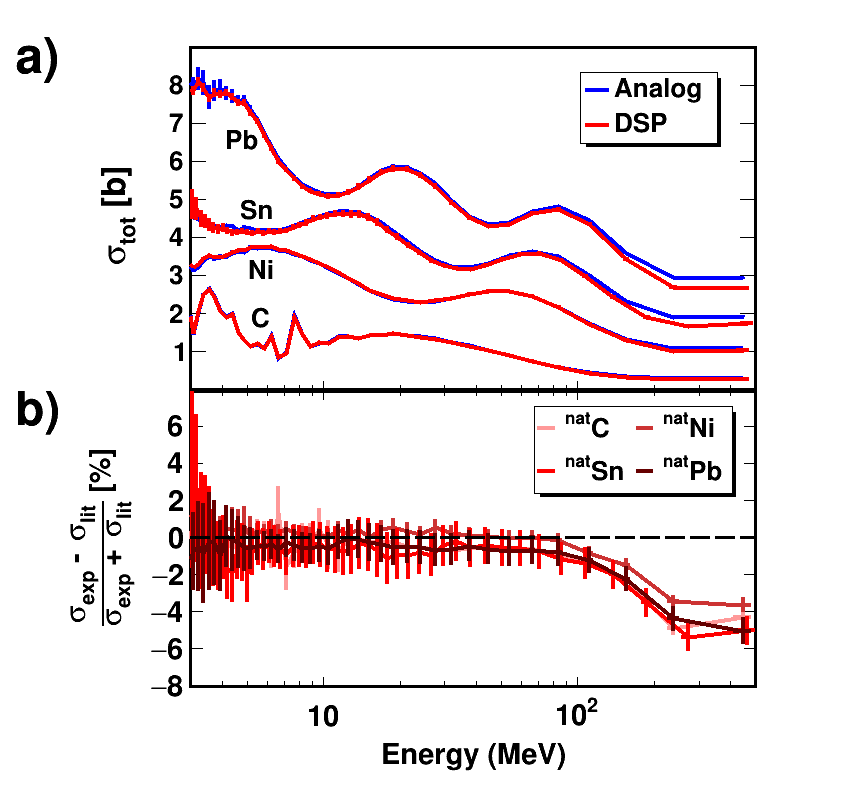
\includegraphics[scale=0.5]{figures/literatureBenchmarking.png}
    \caption{Comparison of our natural-sample \tot\ measurement against literature data}
    \label{LiteratureBenchmarking}
\end{figure*}

(Color online) A comparison of literature data (taken with analog
    techniques) and our results (signals processed with a digitizer, or "DSP")
    for natural C, Ni, Sn, and Pb. In panel a), the absolute cross sections are shown from
    3-500 MeV; in panel b), the relative differences between the literature data and
    our data are shown in percent. From 3-100 MeV, our data are fully consistent with the
    literature datasets but above 100 MeV, a difference arises, peaking at
    $\approx$5\% at 300 MeV.
b

\begin{figure*}
    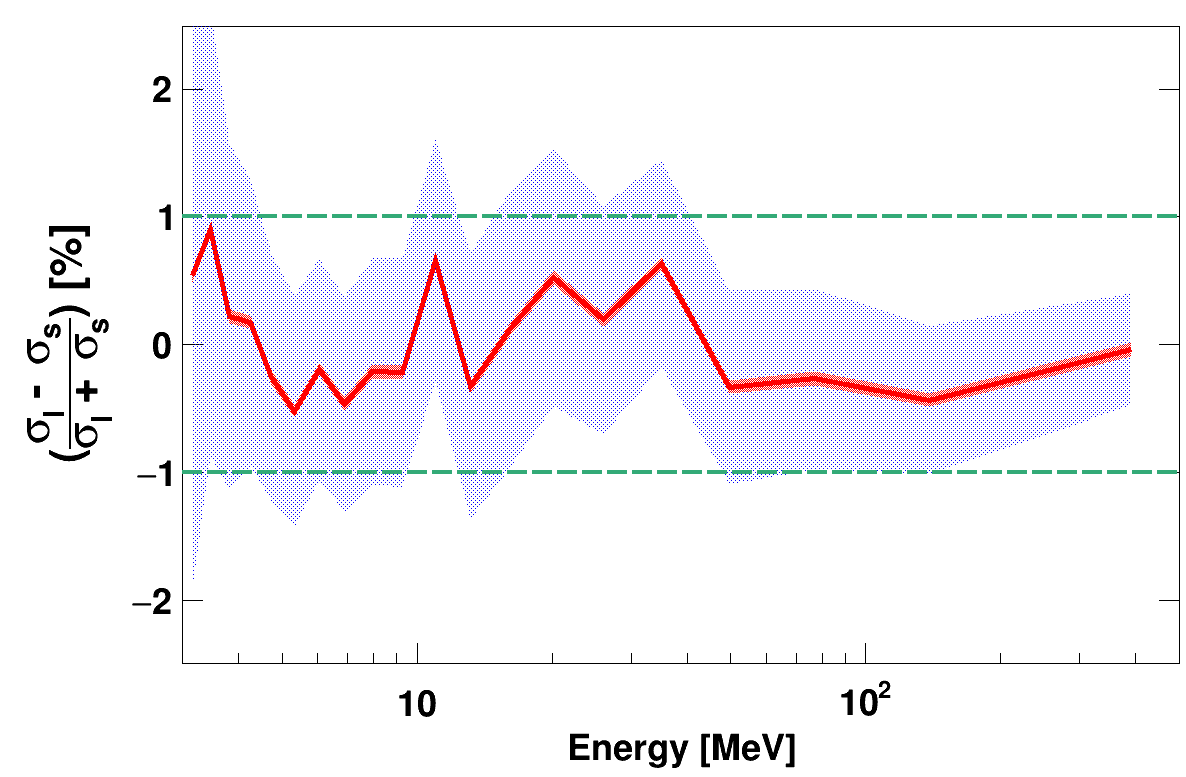
\includegraphics[scale=0.30]{figures/relativeDiff_longCarbonShortCarbon.png}
    \caption{Neutron \tot\ relative difference between short and long \cNat\ samples}
    \label{CarbonBenchmarking}
\end{figure*}

(Color online) Relative difference of cross sections (red line) of
        our two lengths of \cNat, (27.3 mm and 13.7 mm), shown from 3-400
        MeV. Total error
        (including statistical and systematic) is indicated by the blue
        dotted region. Systematic error only (due to uncertainty in the areal
        density) is shown by the red hatched region (very small and immediately adjacent to 
        the red line). Clearly, statistical error dominates for this relative
        difference.
        Despite the low statistics of this diagnostic run (only 1.5 hours
        beam-on-target for each sample), the high efficiency of the
        digitizer-enabled approach means that the relative difference can be resolved to 
        $\pm$1\% for most of the energy range.


Our absolute \tot\ results for all isotopic targets are shown in Figs.
\ref{TwoPanelO, TwoPanelNi, TwoPanelRh, TwoPanelSn}. All previous isotopic \tot\
measurements (where they exist) are shown alongside our results for comparison.
To compare the results, relative differences between our data and literature
data are also plotted below. The literature
data sets shown have been modified to have the same bins as our data via a simple
linear interpolation of the original data's bins. This rebinning
washes out the fine structure of the cross section data where the density of states
for a given sample is low and individual resonances are visible
(e.g., $^{\text{nat}}$C below 10 MeV).

Relative differences of our measured \tot\ between \oSixEight, \niEightFour, and
\snTwelveFour are shown in Figs. \ref{IsotopicDiffO, IsotopicDiffNi, 
IsotopicDiffSn}, respectively. 

\subsection{\oSixEight\ \tot\ results}
\begin{figure*}
    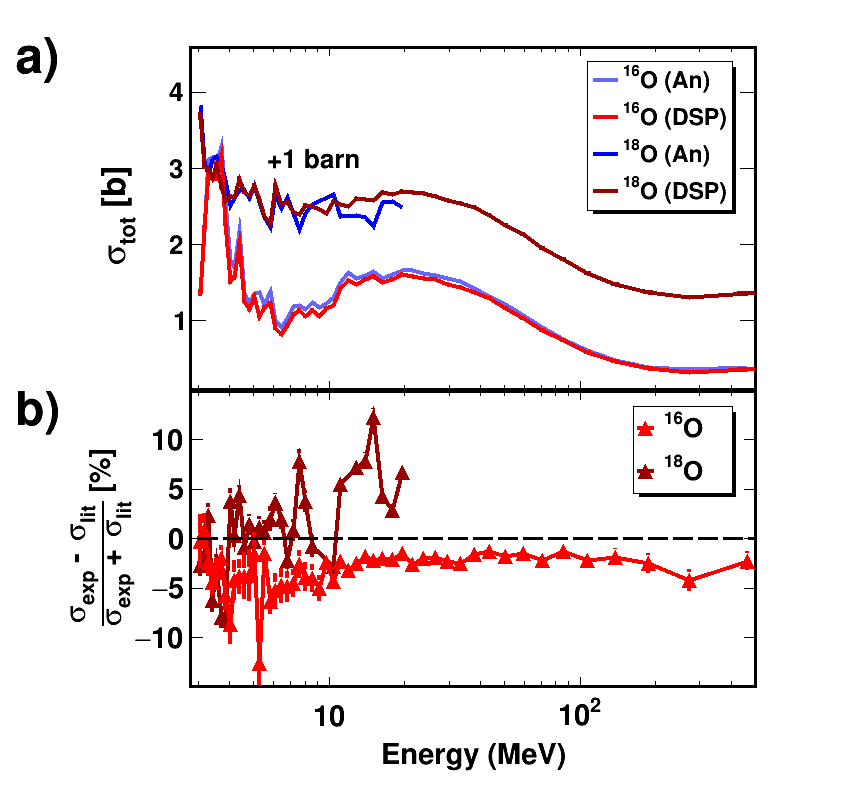
\includegraphics[scale=0.35]{figures/TwoPanelO.png}
    \caption{Neutron \tot\ for \oSixEight: our results and literature data}
    \label{TwoPanelO}
\end{figure*}

        \cite{Finlay1993, Perey1972, Vaughn1965, Salisbury1965}

\begin{figure*}
    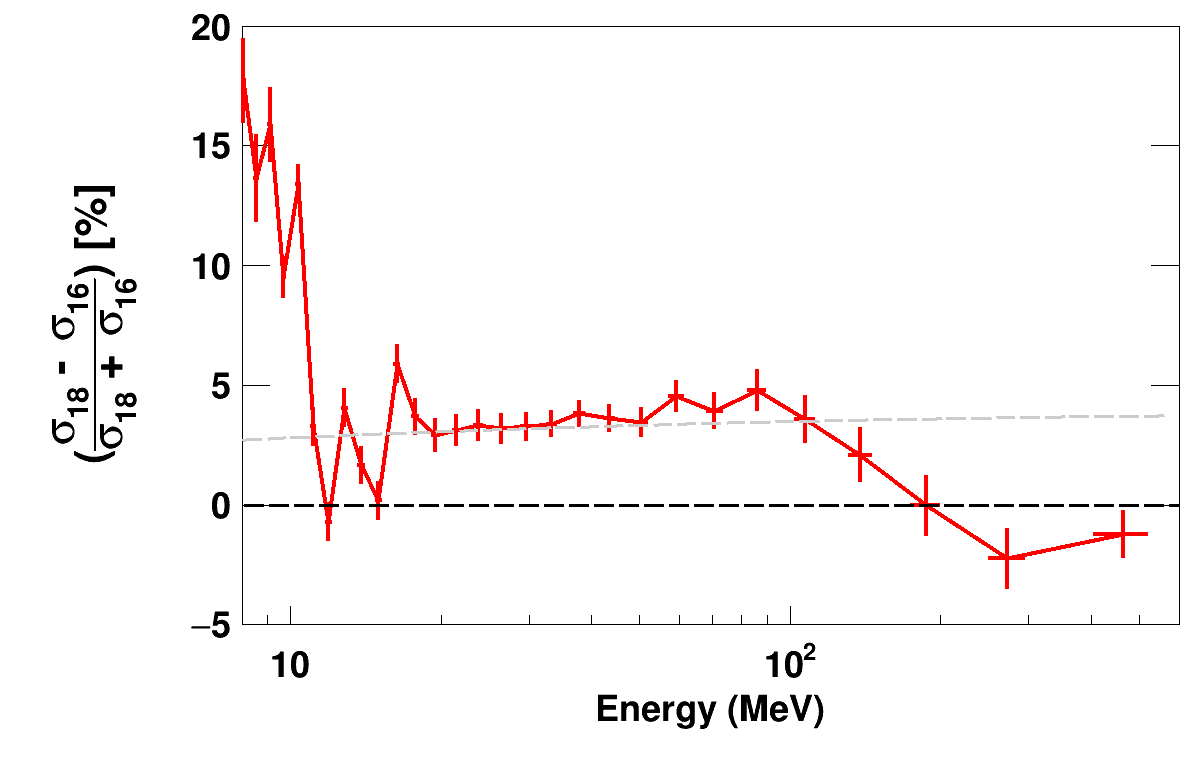
\includegraphics[scale=0.35]{figures/relativeDiff_O18O16.png}
    \caption{\oSixEight\ neutron \tot\ relative difference}
    \label{IsotopicDifferenceO}
\end{figure*}

\subsection{\niEightFour\ \tot\ results}
\begin{figure*}
    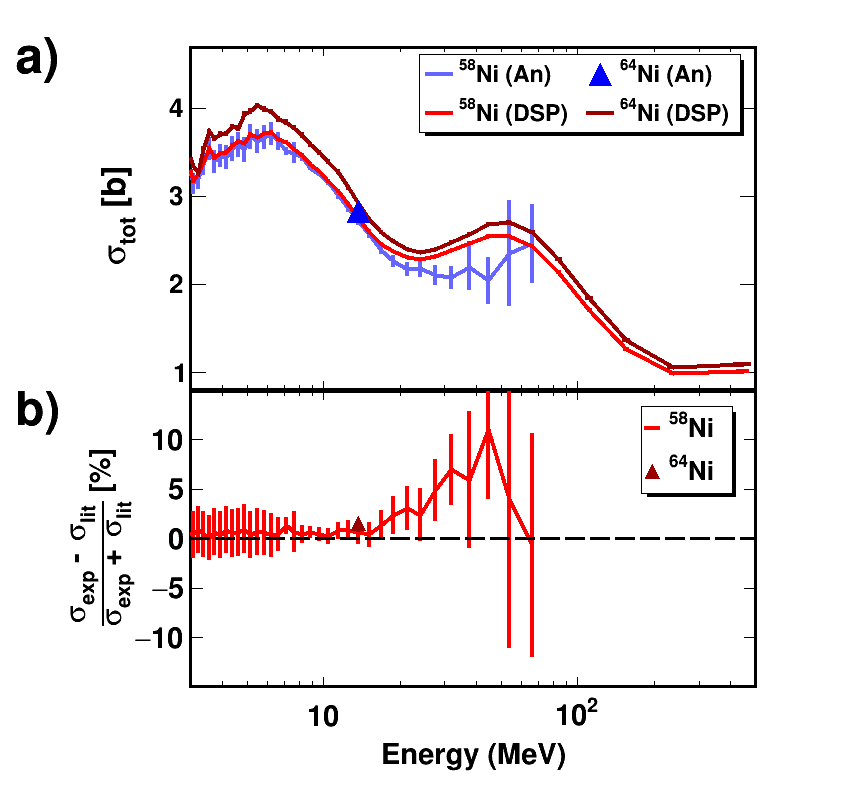
\includegraphics[scale=0.35]{figures/TwoPanelNi.png}
    \caption{Neutron \tot\ for \niEightFour: our results and literature data}
    \label{TwoPanelNi}
\end{figure*}

(Color online) Neutron total cross sections for $^{58,64}$Ni.
        (a) shows our isotopic results (in shades of red) and
        corresponding literature data \cite{Perey1993, Dukarevich1967} (in
        shades of blue). (b) shows the relative difference between our data
        and literature data that are shown in panel a). The reported error in
        the literature data set for $^{58}$Ni is the major contributor to the
        large error bars shown in the $^{58}$Ni relative difference. In this
        energy range, only one data point was available for $^{64}$Ni (indicated
        by the triangles) from Dukarevich's 1967 study of isotopically-resolved cross
        sections at 14.2 MeV \cite{Dukarevich1967}.

\begin{figure*}
    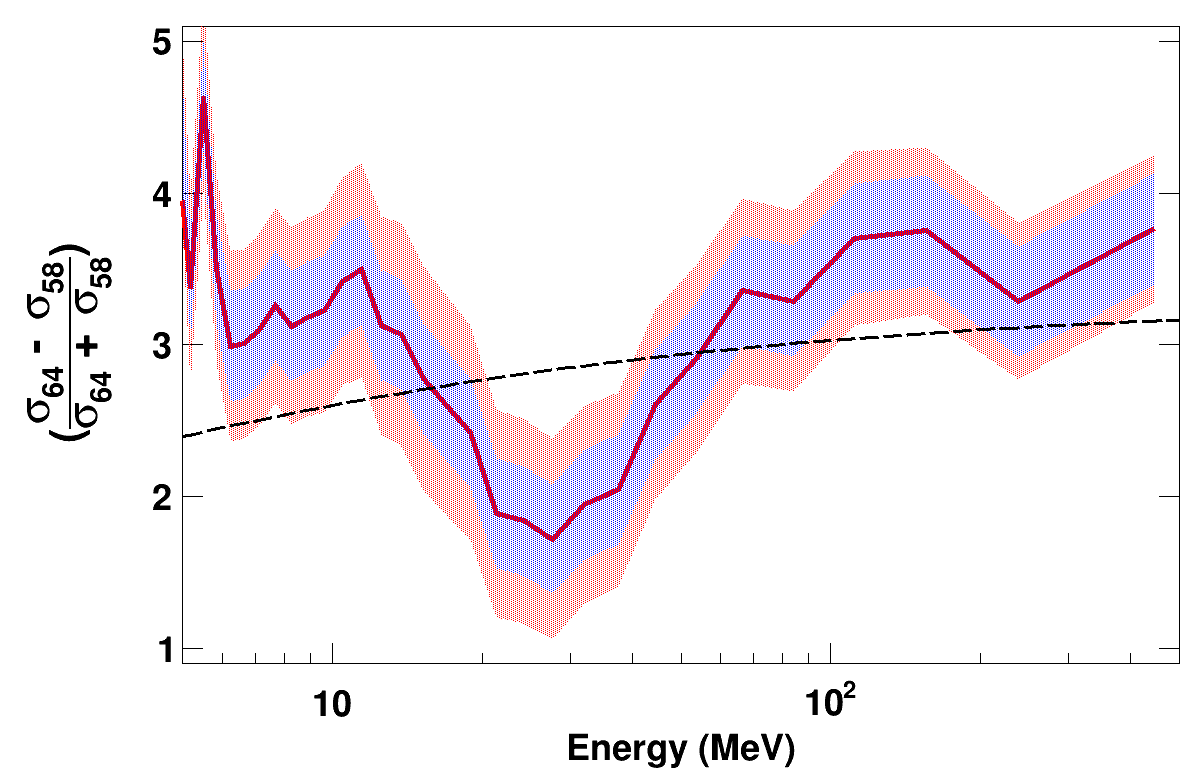
\includegraphics[scale=0.35]{figures/relativeDiff_Ni64Ni58.png}
    \caption{\niEightFour\ neutron \tot\ relative difference}
    \label{IsotopicDifferenceNi}
\end{figure*}

(Color online) Relative difference of cross sections (red line) of
        $^{\text{64}}$Ni and $^{\text{58}}$Ni, shown from 5-400
        MeV. Total error
        (including statistical and systematic) is indicated by the red
        dotted region. Systematic error only (due to uncertainty in the areal
        density) is shown by the blue dotted region. The SAS prediction (Eq.
        \ref{SASRelDiff}) is shown by the black dashed line.

\subsection{\rhThree\ \tot\ results}
\begin{figure*}
    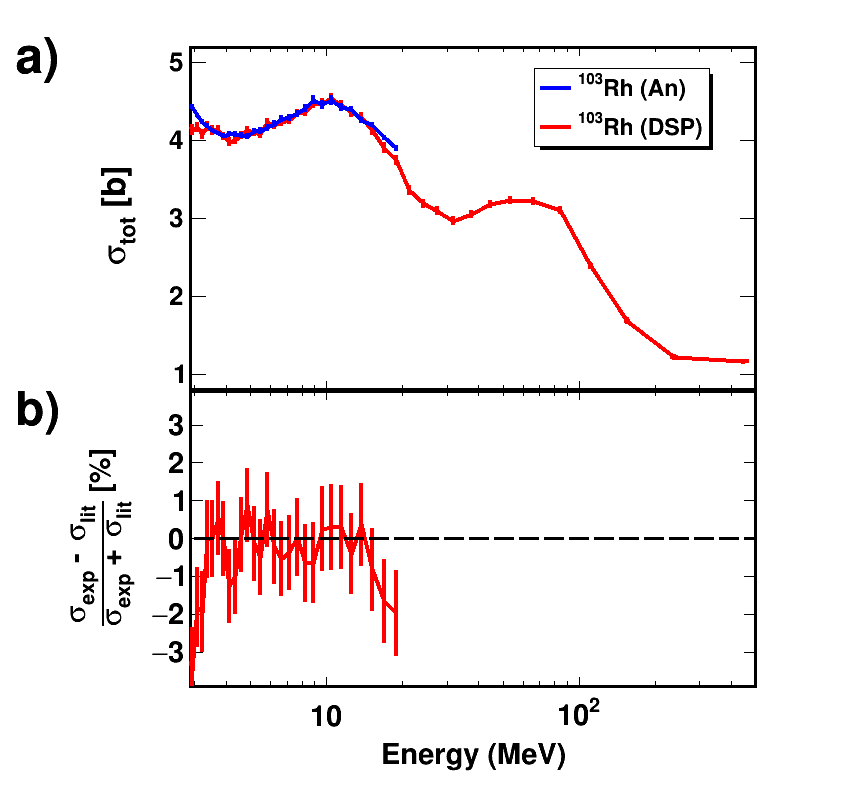
\includegraphics[scale=0.35]{figures/TwoPanelRh.png}
    \caption{Neutron \tot\ for \rhThree: our results and literature data}
    \label{TwoPanelRh}
\end{figure*}

        \cite{Poenitz1983}

\subsection{\snTwelveFour\ \tot\ results}
\begin{figure*}
    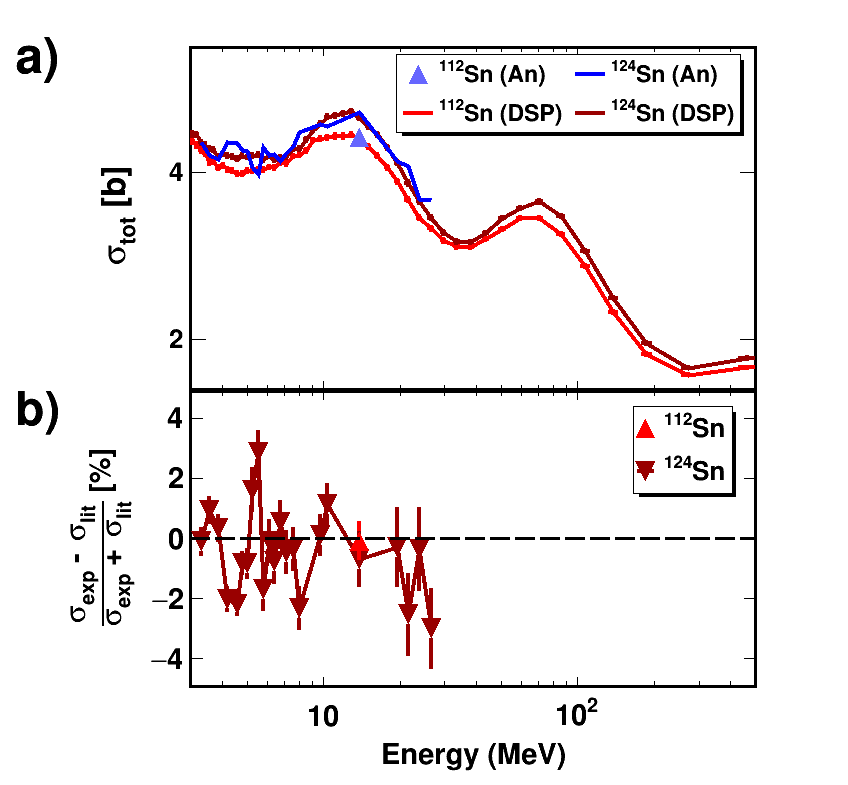
\includegraphics[scale=0.35]{figures/TwoPanelSn.png}
    \caption{Neutron \tot\ for \snTwelveFour: our results and literature data}
    \label{TwoPanelSn}
\end{figure*}

(Color online) Neutron total cross sections for $^{112,124}$Sn.
        (a) shows our isotopic results (in shades of red) and
        corresponding literature data \cite{Harper1982, Timokhov1989, Rapaport1980, Dukarevich1967} (in
        shades of blue). (b) shows the relative difference between our data
        and literature data that are shown in panel a). The data sets are in
    excellent agreement where literature data exists (up to $\approx$20 MeV).

\begin{figure*}
    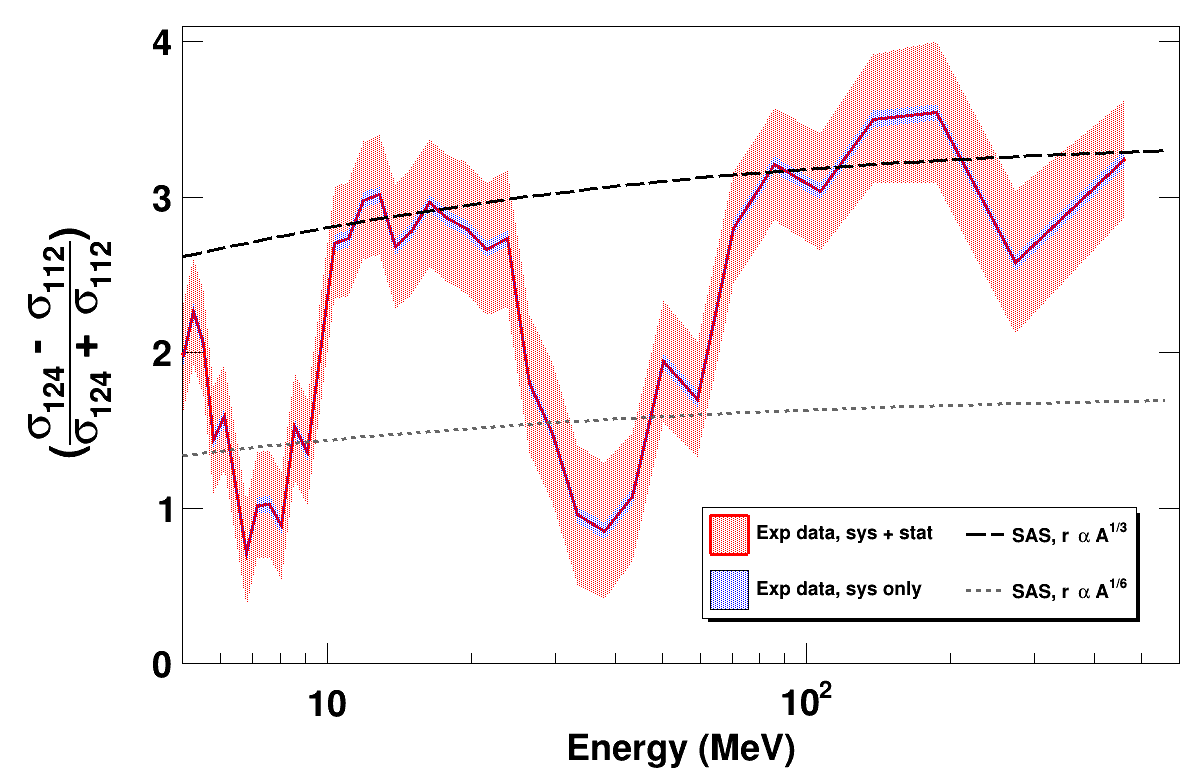
\includegraphics[scale=0.35]{figures/relativeDiff_Sn124Sn112.png}
    \caption{\snTwelveFour\ neutron \tot\ relative difference}
    \label{IsotopicDifferenceSn}
\end{figure*}

\afterpage{\clearpage}
